\chapter{זמן מסך ורווחה}
\label{ch:wellbeing}

\begin{epigraph}{}
התרופה והרעל עשויים לעיתים קרובות מאותו חומר. ההבדל הוא במינון.
\end{epigraph}

\section{הדייסה של זהבה}

באגדה הבריטית הישנה, ילדה בשם זהבה (\en{Goldilocks}) נכנסת לבית של שלושה דובים. היא טועמת מהדייסה שלהם: אחת חמה מדי, אחת קרה מדי, והשלישית בדיוק כמו שצריך. האגדה נועדה לילדים, אבל היא מכילה רעיון שמדענים אוהבים מאוד: לפעמים התשובה הנכונה איננה "כן" או "לא", אלא "בערך באמצע".

השיח הציבורי על מסכים נוטה לשכוח את זה. כותרות העיתונים מחולקות בדרך כלל לשני מחנות. מחנה אחד טוען שהסמארטפון הורס דור שלם. המחנה השני טוען שזו בהלה מוסרית, כמו זו שליוותה בעבר את הרומן, את הרדיו ואת הקומיקס. ומה אומרים הנתונים? כצפוי, משהו מסובך יותר.

\section{מה מצאו באוקספורד}

ב-2017 פרסמו אנדרו פשיבילסקי ונטע וינשטיין מחקר על 120,115 מתבגרים באנגליה, מדגם גדול במיוחד \parencite{przybylski2017}. הם לא שאלו רק "האם מסכים מזיקים?", אלא "בכמה שימוש, ובאיזה סוג?". ההשערה שלהם קיבלה את השם \textbf{השערת גולדילוקס}: שימוש מתון בטכנולוגיה דיגיטלית אינו מזיק מטבעו, ואף עשוי להועיל בעולם מחובר, ורק שימוש מוגזם קשור לירידה ברווחה.

והנתונים אכן הראו צורה של \textbf{U הפוכה}. הרווחה הנפשית עלתה עם שימוש מתון, הגיעה לשיא, ומשם התחילה לרדת. כל פעילות הגיעה לנקודת המפנה שלה בזמן אחר, והתמונה השתנתה בין ימי חול לסופי שבוע \parencite{przybylski2017}.

\section{מודל גולדילוקס}

כדי לראות את הרעיון בבירור, נבנה מודל מתמטי פשוט. חשוב להדגיש: הנוסחה שלהלן היא \textbf{המחשה} שהספר הזה בונה כדי להסביר את צורת הממצא. זו איננה נוסחה שמצוטטת מתוך המאמר.

\begin{eqbox}[מודל גולדילוקס: רווחה כפונקציה של זמן מסך]
\begin{equation}
W(t) = \beta_0 + \beta_1 t - \beta_2 t^2
\label{eq:goldilocks}
\end{equation}
\end{eqbox}

מה אומר כל סימן במשוואה~\eqref{eq:goldilocks}?

\begin{itemize}
  \item $W$ היא \textbf{הרווחה הנפשית} (\en{Well-being}), כפי שהיא נמדדת בשאלון.
  \item $t$ הוא מספר \textbf{שעות המסך היומיות} בפעילות מסוימת.
  \item $\beta_0$ היא רמת הרווחה הבסיסית, כשאין שימוש כלל.
  \item $\beta_1 > 0$ מתאר את התועלת של השימוש: קשר עם חברים, מידע, הנאה. זה האיבר שמושך את העקומה למעלה.
  \item $\beta_2 > 0$ מתאר את המחיר שמצטבר: שינה שנגמרה מוקדם, פעילות גופנית שנדחתה, השוואה מתמדת לאחרים. בגלל הריבוע $t^2$, המחיר הזה גדל מהר יותר מהתועלת, ובסוף מנצח.
\end{itemize}

איפה נמצא השיא? בנקודה שבה העקומה מפסיקה לעלות ומתחילה לרדת, כלומר כשהנגזרת שווה לאפס:
\[
\frac{dW}{dt} = \beta_1 - 2\beta_2 t = 0
\]
ומכאן נקודת האופטימום:
\begin{equation}
t^{*} = \frac{\beta_1}{2\beta_2}
\label{eq:optimum}
\end{equation}

משוואה~\eqref{eq:optimum} אומרת משהו אינטואיטיבי: ככל שהתועלת $\beta_1$ גדולה יותר, נקודת המפנה מתרחקת. ככל שהמחיר $\beta_2$ כבד יותר, היא מתקרבת. למשל, אם $\beta_1 = 2$ ו-$\beta_2 = 0.5$, אז $t^{*} = 2$ שעות ביום. אלה מספרים להמחשה בלבד, אבל הם מראים למה אין "מספר קסם" אחד לכל המסכים.

% גרף Python: python/make_graphs.py → images/goldilocks.png
\begin{figure}[htbp]
\centering
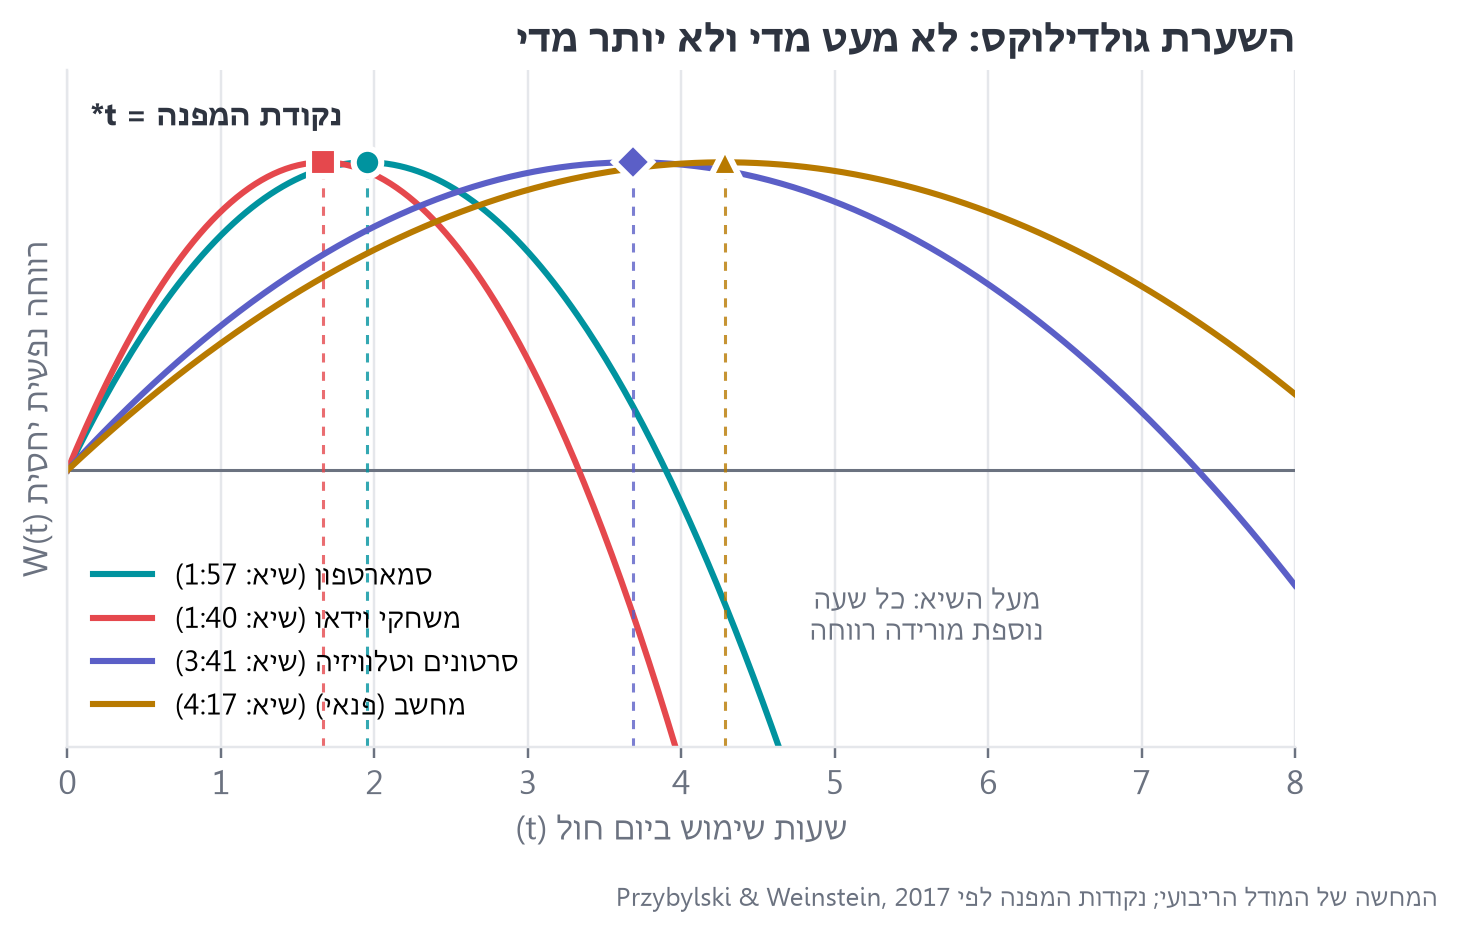
\includegraphics[width=0.92\textwidth]{images/goldilocks.png}
\caption[המחשה של מודל גולדילוקס: נקודת מפנה לכל פעילות]{המחשה של מודל גולדילוקס (משוואה~\ref{eq:goldilocks}): לכל פעילות יש נקודת מפנה $t^{*}$ משלה. נקודות המפנה לימי חול לפי \textcite{przybylski2017}. העקומות בנויות כך שהשיא ייפול על נקודת המפנה, והגובה השווה שלהן הוא נרמול: הן מראות \textbf{איפה} השיא, לא כמה הוא גבוה. האפקט שנמדד בפועל קטן \parencite{orben2019}.}
\label{fig:goldilocks}
\end{figure}


איור~\ref{fig:goldilocks} מציג ארבע עקומות להמחשה, אחת לכל פעילות, וכל אחת מגיעה לשיא בנקודת המפנה שדווחה עבור ימי חול \parencite{przybylski2017}:

\begin{itemize}
  \item \textbf{סמארטפון}: כשעה ו-57 דקות ביום.
  \item \textbf{משחקי וידאו}: כשעה ו-40 דקות ביום (ובסוף השבוע כ-3 שעות ו-35 דקות).
  \item \textbf{צפייה בסרטונים ובטלוויזיה}: כ-3 שעות ו-41 דקות ביום (ובסוף השבוע כ-4 שעות ו-50 דקות).
  \item \textbf{מחשב לשימוש פנאי}: כ-4 שעות ו-17 דקות ביום.
\end{itemize}

במילים פשוטות: בערך שעתיים בסמארטפון ביום חול, ועד כארבע שעות ויותר בצפייה וביישומי מחשב. הסמארטפון, המכשיר הקרוב ביותר לגוף, ומשחקי הווידאו מגיעים לנקודת המפנה מהר ביותר, עוד לפני שתי שעות ביום.

\begin{alertbox}[זהירות: אפקט קטן, קשר ולא סיבה]
שני דברים חשוב לזכור. ראשית, \textbf{האפקט חלש}. גם בשימוש גבוה, ההבדל ברווחה קטן \parencite{przybylski2017}. שנית, זה \textbf{מחקר מתאמי}: הוא מראה ששני דברים הולכים יחד, לא שאחד גורם לשני. ייתכן שמתבגרים שמרגישים רע פונים יותר למסכים, ולא להפך. ניתוח מאוחר יותר של מדגמים גדולים מצא קשר שלילי קטן מאוד בין שימוש בטכנולוגיה לבין רווחת מתבגרים \parencite{orben2019}.
\end{alertbox}

\section{ויכוח אמיתי}

כאן נכנס לתמונה הוויכוח הסוער ביותר בתחום. הפסיכולוג החברתי ג'ונתן הייט טוען שבין 2010 ל-2015 בערך התרחשה \en{the Great Rewiring of Childhood}, "החיווט מחדש הגדול של הילדות": מעבר מילדות שמבוססת על משחק לילדות שמבוססת על טלפון. לדבריו, זה גורם מרכזי במשבר בריאות הנפש של בני נוער \parencite{haidt2024}.

מנגד, איימי אורבן ואנדרו פשיבילסקי מזהירים מהכללות רחבות. לפי הניתוח שלהם, הקשר הממוצע בין טכנולוגיה דיגיטלית לרווחה הוא שלילי, אבל קטן מאוד, ואין להפוך אותו לסיפור של קטסטרופה \parencite{orben2019}.

מי צודק? ייתכן ששניהם, חלקית. ממוצעים קטנים יכולים להסתיר קבוצות שנפגעות מאוד. ומצד שני, בהלה מוסרית יכולה להסיט את תשומת הלב מגורמים אחרים, כמו לחץ בלימודים, מצב כלכלי או בדידות. זה לא ויכוח בין מדע לבורות. זה ויכוח בתוך המדע, והוא עדיין לא הוכרע.

\begin{thinkbox}
אם ההבדל הממוצע קטן, האם זה אומר שאין בעיה? או שמא בעיה קטנה אצל מיליארד אנשים היא, בסופו של דבר, בעיה גדולה מאוד?
\end{thinkbox}
